\documentclass[10pt,a4paper,table]{article}
	
	\usepackage{amsmath,amssymb,amsthm,mathtools,amsfonts}
	\usepackage{breqn}
	\usepackage[utf8]{inputenc}
	\usepackage[danish]{babel}
	\usepackage[T1]{fontenc}
	
	%%%%%%%%%%%%%%%%%%%%%%%%%%%%%%%%%%%%%%%%%%%%%%%%%%%%%%%%%%%%%%%%%%%%%%%%%%%%%% Fonts
	
	\usepackage{fontspec}
	\setmainfont{Times New Roman}
	\newfontfamily\garamond[Numbers=OldStyle]{EB Garamond}
	\newfontfamily\plantin[Numbers=OldStyle]{Plantin MT Pro}
	\newfontfamily\wal{Walbaum Com}
	\newfontfamily\klav{Klavika}
	\newfontfamily\klavl{Klavika light}
	\newfontfamily\quotefont[Ligatures=TeX]{Linux Libertine O}
	\newfontfamily\vest{TRY Vesterbro Regular}
	\newfontfamily\vestb{TRY Vesterbro Poster}
	\newfontfamily\overp{Overpass}
	
	%%%%%%%%%%%%%%%%%%%%%%%%%%%%%%%%%%%%%%%%%%%%%%%%%%%%%%%%%%%%%%%%%%%%%%%%%%%%%% Colors
	
	\usepackage{xcolor}
	
	\definecolor{frbblue}{RGB}{47, 88, 109}
	\definecolor{hgred}{RGB}{140, 10, 10}
	\definecolor{frbgreenl}{RGB}{162, 202, 137}
	\definecolor{frbgreen}{RGB}{28, 85, 66}
	\definecolor{frbgrey}{RGB}{243, 245, 242}
	
	%%%%%%%%%%%%%%%%%%%%%%%%%%%%%%%%%%%%%%%%%%%%%%%%%%%%%%%%%%%%%%%%%%%%%%%%%%%%%% Other Graphics
	
	\usepackage{graphicx}
	\graphicspath{{../img/}}
	\usepackage{tikz}
	\usepackage{placeins}
	\usepackage{subcaption}
	
	\usepackage[pdfborder={0 0 0}]{hyperref} %% Ingen firkant rundt om referencer

	\usepackage{multicol}
	\usepackage{cellspace}
		\setlength\cellspacetoplimit{100pt}
		\setlength\cellspacebottomlimit{100pt}
	\usepackage{tabularx}
		\newcolumntype{b}{>{\hsize=\hsize}>{\centering\arraybackslash}X}
	\usepackage{siunitx}
	\usepackage{cellspace}
		\setlength\cellspacetoplimit{4pt}
		\setlength\cellspacebottomlimit{4pt}
	
	\usepackage{enumitem}% better controls with enumerating
	\usepackage{wrapfig}
	\usepackage{caption}
	%\usepackage{dirtytalk}
	%\usepackage{tasks}
	\usepackage{titlesec}

	\setlength{\parskip}{0.5\baselineskip}
	\setlength{\parindent}{0cm}
	\setlist[enumerate]{label=\alph*),left=20pt}
	%\setlist[enumerate]{leftmargin=\parindent}
	%\setlist[enumerate]{nosep}
	
	
	%%%%%%%%%%%%%%%%%%%%%%%%%%%%%%%%%%%%%%%%%%%%%%%%%%%%%%%%%%%%%%%%%%%%%%%%%%%%%% New commands
	
	\newcommand\svar[1]{\newline\textcolor{red}{\textbf{Svar}\\#1}}
	
	\usepackage[h]{esvect}
	\newcommand{\twvect}[2]{\ensuremath{\begin{pmatrix}#1\\#2\end{pmatrix}}}
	
	\newcommand*\quotesize{20}
	\newcommand*{\openquote}
		{\tikz[remember picture,overlay,xshift=-3ex,yshift=-0ex]
			\node (OQ) {\quotefont\fontsize{\quotesize}{\quotesize}\selectfont``};\kern0pt}

	\newcommand*{\closequote}[1]
		{\tikz[remember picture,overlay,xshift=2ex,yshift={#1}]
			\node (CQ) {\quotefont\fontsize{\quotesize}{\quotesize}\selectfont''};}
			
	\newcommand{\qm}[1]{``#1''}
	\newcommand{\iquote}[1]{\begin{quote}\itshape \openquote#1\hfill\closequote{0ex} \end{quote}}
	
	%%%%%%%%%%%%%%%%%%%%%%%%%%%%%%%%%%%%%%%%%%%%%%%%%%%%%%%%%%%%%%%%%%%%%%%%%%%%%% Sections
	\usepackage{chngcntr}
	
	\renewcommand\thesection{\arabic{section}}

	\titleformat{\section}[block] 
  		{\flushright\overp\Large\color{frbgreen}}    % format for whole title
  		{}                           % no separate label (empty)
  		{0pt}                        % spacing between label and title
		{DELPRØVE \thesection}       % prepend "Delprøve <number>"
		[{\color{frbgreenl}\vspace{-1em}\hspace*{-0.165\linewidth}\rule{\dimexpr1.165\linewidth\relax}{0.4pt}\kern1mm}]
	
	\counterwithout{subsection}{section}
	\renewcommand\thesubsection{Opgave \arabic{subsection}}
	\titleformat{\subsection}[leftmargin]{\bfseries}{}{0pt}{\hspace{-5em}\thesubsection}
	
	%%%%%%%%%%%%%%%%%%%%%%%%%%%%%%%%%%%%%%%%%%%%%%%%%%%%%%%%%%%%%%%%%%%%%%%%%%%%%% Header & Footer
	
	\usepackage{bigfoot}
	\DeclareNewFootnote{a}
		\renewcommand{\thefootnotea}{\fnsymbol{footnotea}}
			\newcommand{\footnotes}[1]{\footnotea[2]{#1}} % here you can specify what symbol you want in footnotes
			\MakePerPage{footnotes}
	
		\usepackage{fancyhdr}
	\fancypagestyle{plain}{%
		\setlength{\headheight}{60pt}%
		\setlength{\headsep}{0pt}
		\fancyhf{}% No header/footer
		\renewcommand{\footrulewidth}{0pt}% No footer rule
		\renewcommand\headrule{
			\centerline{\begin{minipage}{1\textwidth}
				\color{frbblue}\hrule width \hsize \kern 1mm \hrule width \hsize height 2pt \vspace{4em}
			\end{minipage}}
		}
		\fancyhead[L]{\hspace{0em}
\includegraphics[height=2.5em]{frbvuc_logo.png}}
		\fancyhead[R]{\overp\color{frbgreen}\footnotesize Forår 2026}
		\fancyhead[C]{\overp\color{frbgreenl}\normalsize \overp Mat C-B\\\Large\color{frbgreen}\vestb Aflevering 9}
		\cfoot{\thepage}
	}
	\pagestyle{fancy}
	\fancyhf{}
	\renewcommand\headrule{
			\centerline{\begin{minipage}{\textwidth}
				\color{frbgreen}\hrule width \hsize \kern 1mm
			\end{minipage}}}
	\lhead{\overp\color{frbgreen}\footnotesize Mat C-B}
	\rhead{\overp\color{frbgreen}\footnotesize Forår 2026}
	\cfoot{\thepage}
	
	%%%%%%%%%%%%%%%%%%%%%%%%%%%%%%%%%%%%%%%%%%%%%%%%%%%%%%%%%%%%%%%%%%%%%%%%%%%%%% Document

\begin{document}
\thispagestyle{plain}

\section{}
\subsection{}
\
\begin{figure}[h!]
\centering
\vspace{-15pt}
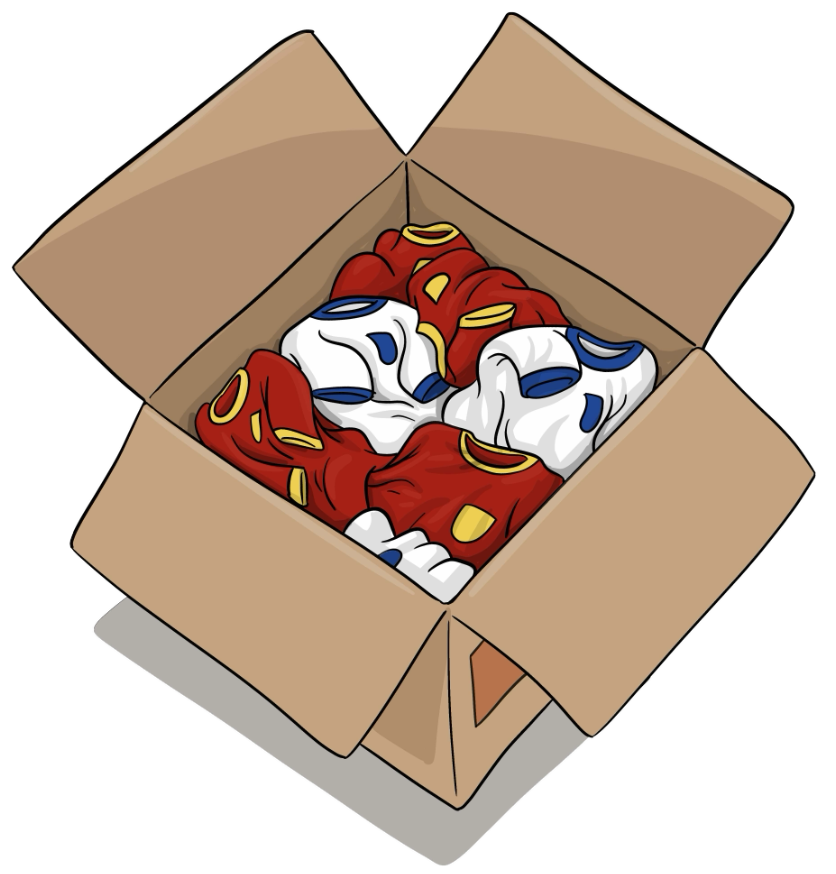
\includegraphics[width=0.35\textwidth]{jersey.png}
\end{figure}

Fra en kasse med 8 fodboldtr\o jer tr\ae kkes tilf\ae ldigt 2 tr\o jer. R\ae kkef\o lgen har ikke betydning.

\begin{enumerate}
    \item Bestem $K(8,2)$, alts\aa{} antal mulige m\aa der de 2 tr\o jer kan v\ae lges p\aa{}.
\end{enumerate}

Det oplyses, at 5 af tr\o jerne i kassen er r\o de.

\begin{enumerate}
    \setcounter{enumi}{1}
    \item Bestem sandsynligheden for, at der v\ae lges 2 r\o de tr\o jer fra kassen.
\end{enumerate}

\subsection{}
Tabellen viser sandsynlighedsfordelingen for en stokastisk variabel $X$.

\begin{figure}[h!]
\centering\renewcommand{\arraystretch}{1.5}
\begin{tabularx}{0.9\textwidth}{|b|b|b|b|b|}
    \hline $x_i$ & 3 & 5 & 7 & 10 \\\hline
    $P(X=x_i)$ & 0,35 & 0,10 & 0,40 & $p$ \\\hline
\end{tabularx}
\end{figure}

\begin{enumerate}
    \item Bestem tallet $p$.
\end{enumerate}

\subsection{}
\
\begin{figure}[h!]
\centering
\vspace{-15pt}
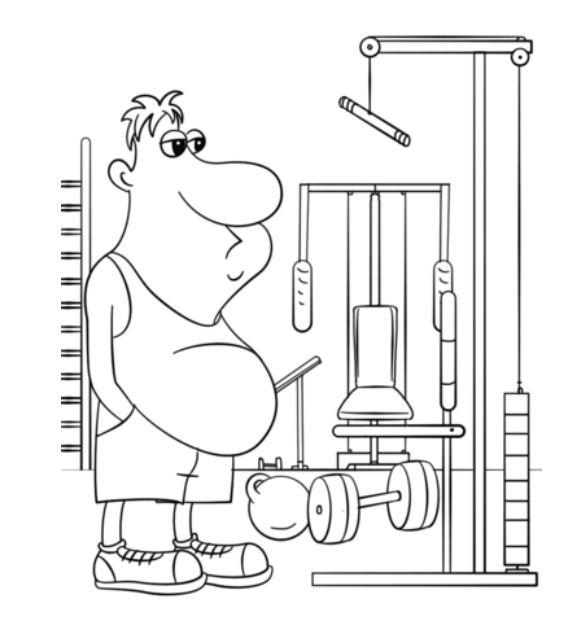
\includegraphics[width=0.35\textwidth]{flemming.png}
\end{figure}

Flemming træner i det lokale fitnesscenter.

Han kender 6 forskellige øvelser for arme og 4 forskellige øvelser for ben.

\begin{enumerate}
    \item På hvor mange måder kan Flemming vælge 3 forskellige øvelser for arme og 2 forskellige øvelser for ben, hvis rækkefølgen af øvelserne ikke har nogen betydning?
\end{enumerate}

\subsection{}
Tabellen viser sandsynlighedsfordelingen for en stokastisk variabel $X$.

\begin{figure}[h!]
\centering\renewcommand{\arraystretch}{1.5}
\begin{tabularx}{0.9\textwidth}{|b|b|b|b|b|}
    \hline $t$ & 1 & 3 & 4 & 6 \\\hline
    $P(X=t)$ & 0,2 & 0,5 & 0,2 & 0,1 \\\hline
\end{tabularx}
\end{figure}

\begin{enumerate}
    \item Bestem $P(X \geq 4)$.
    \item Bestem middelværdien for $X$.
\end{enumerate}

%\clearpage
\section{}
\subsection{}
\begin{wrapfigure}[8]{r}{0.33\textwidth}
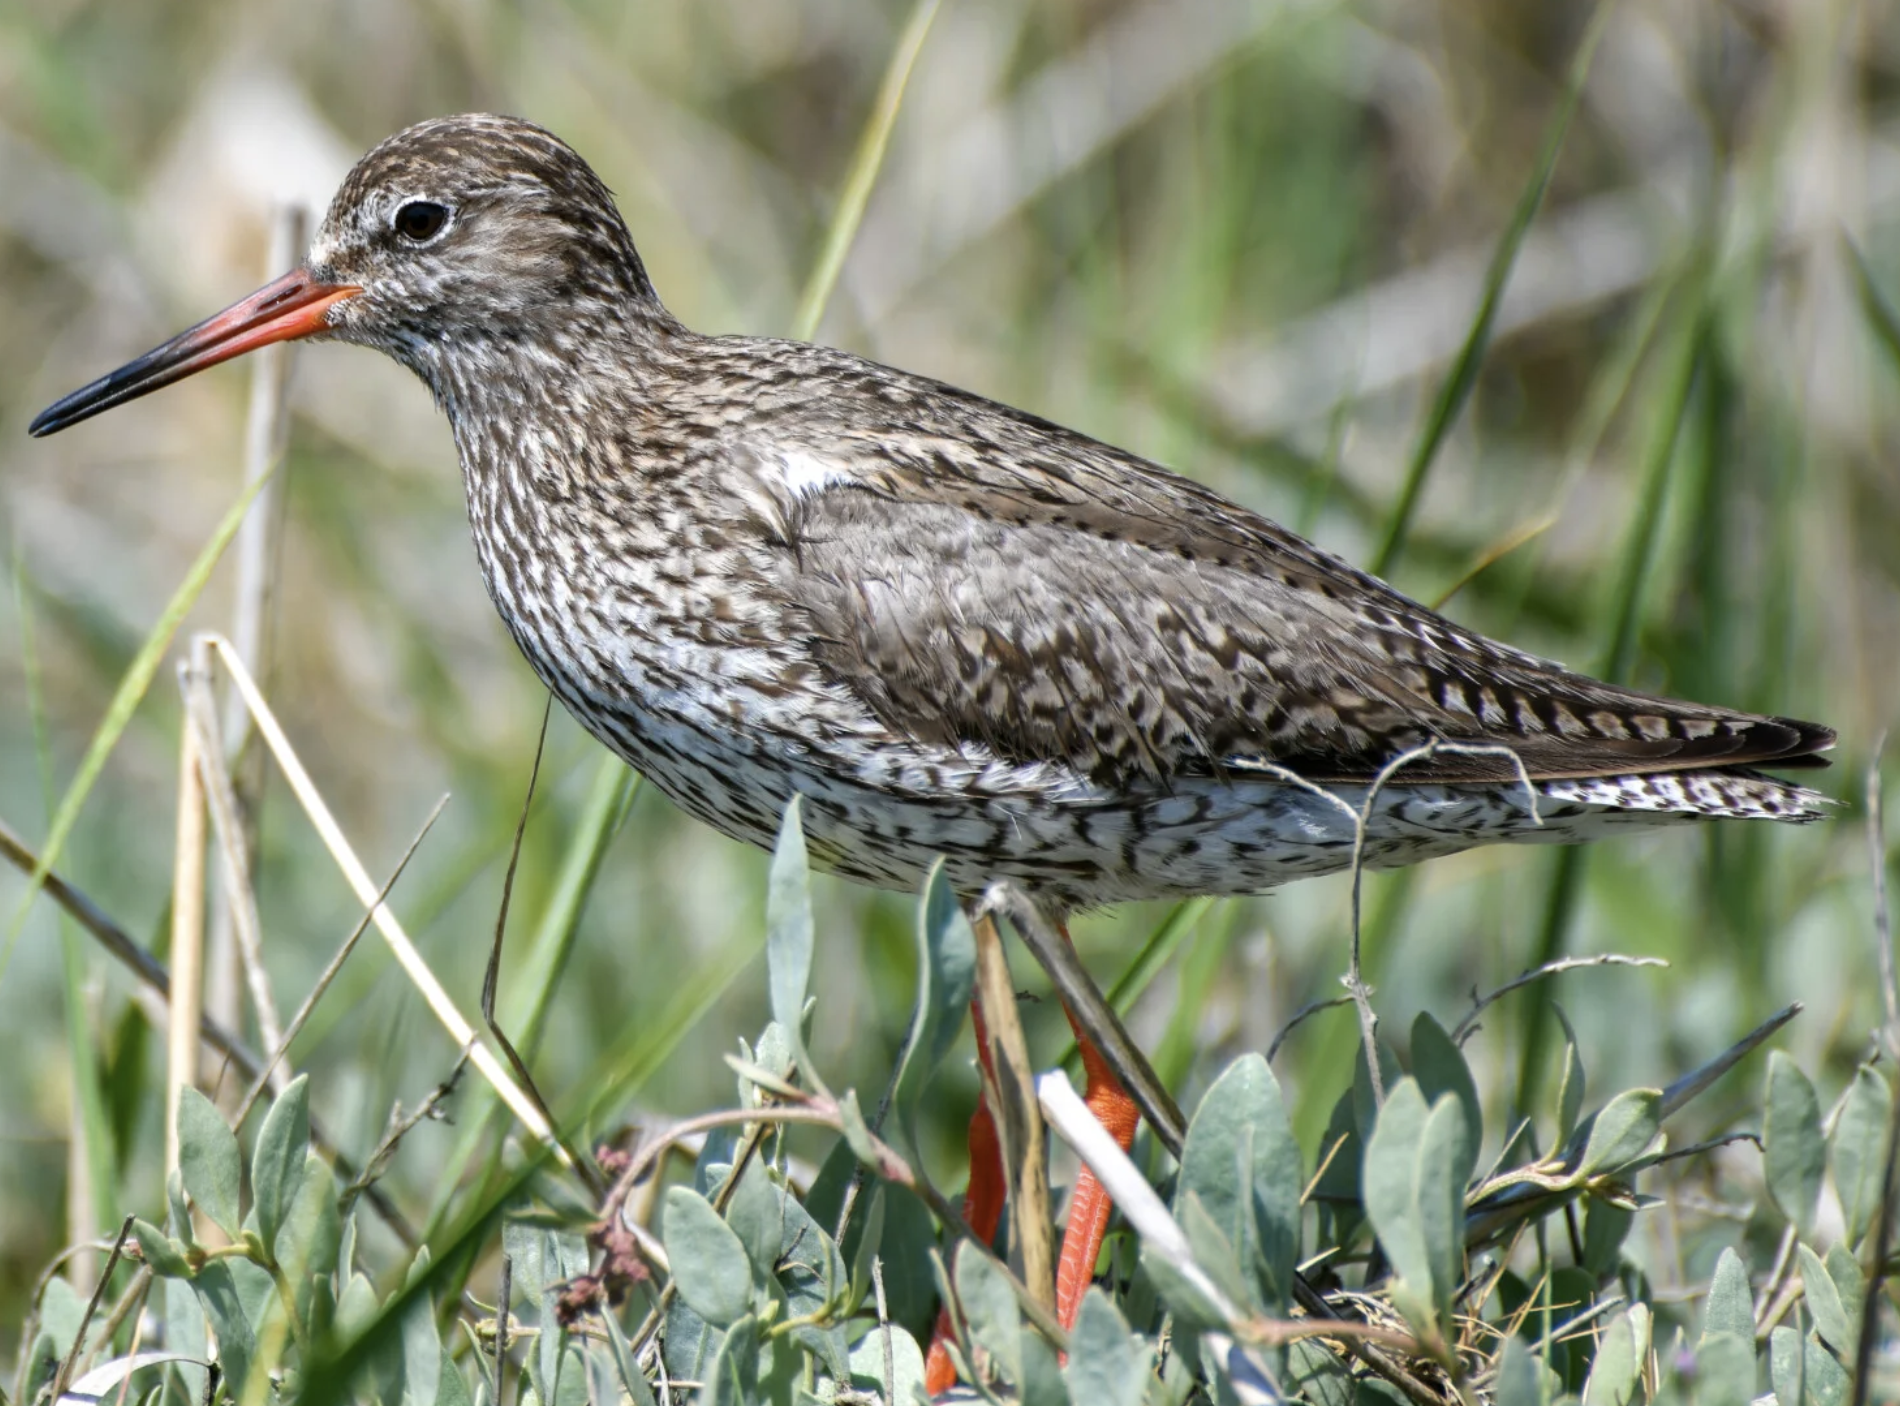
\includegraphics[width=0.5\textwidth]{vogel.png}
\end{wrapfigure}
En unders\o gelse af fuglelivet ved Vadehavet har vist, at sandsynligheden for, at en r\o dbens rede bliver plyndret af rovdyr, er 74\,\%.
I en model betegner den stokastiske variabel $X$ antallet af r\o dbens-reder, der bliver plyndret, blandt 41 reder.
Det antages, at $X$ er binomialfordelt med antalsparameter $n=41$ og sandsynlighedsparameter $p=0,74$.
\begin{enumerate}
    \item Bestem sandsynligheden $P(X \geq 35)$.
    \item Bestem det mest sandsynlige antal reder, der bliver plyndret af rovdyr.
\end{enumerate}

\subsection{}
En stokastisk variabel $X$ er binomialfordelt med antalsparameter $n=85$ og sandsynlighedsparameter $p=0,31$.

\begin{enumerate}
    \item Bestem middelværdien $\mu$ af $X$.
    \item Bestem spredningen $\sigma$ af $X$. Undersøg, om $X=42$ er et exceptionelt udfald for $X$.
\end{enumerate}

\subsection{}
\begin{wrapfigure}[5]{r}{0.33\textwidth}
\vspace{-18pt}
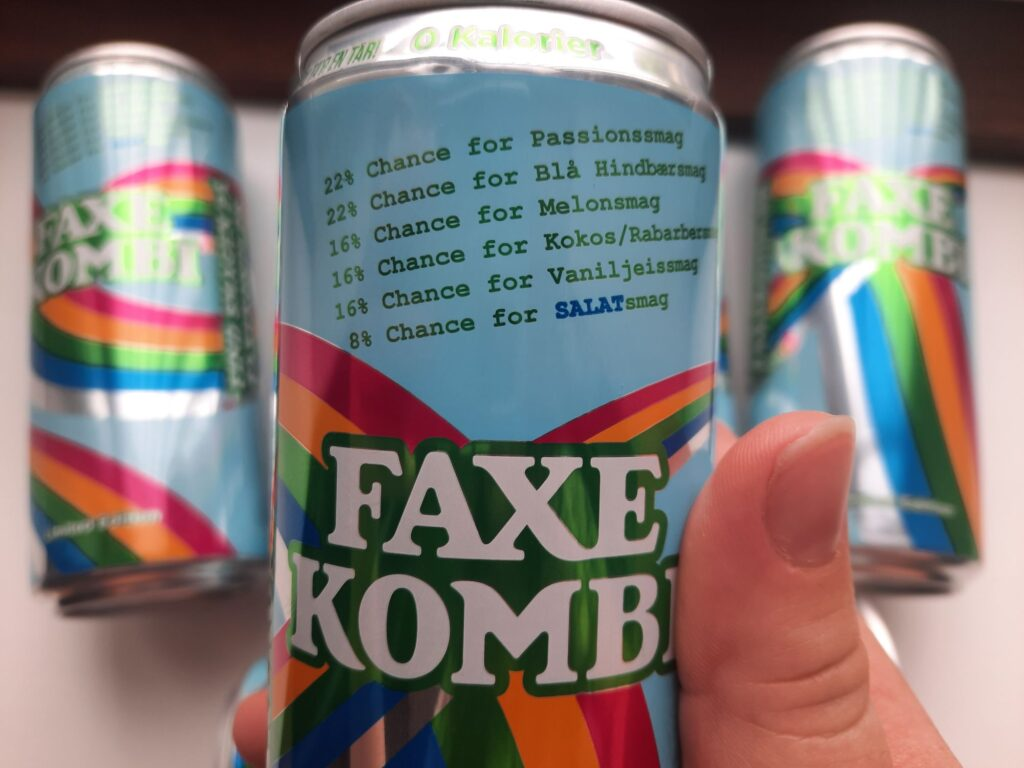
\includegraphics[width=0.5\textwidth]{faxe.png}
\end{wrapfigure}

På en dåse FAXE KOMBI sodavand fremgår det ikke, hvad indholdet smager af.

Der er en sandsynlighed på 8\,\% for, at en sådan dåse indeholder sodavand med smag af salat.

Christian køber 32 dåser FAXE KOMBI.

Den stokastiske variabel $X$ betegner antallet af dåser, som indeholder sodavand med smag af salat. Det antages, at $X$ er binomialfordelt med antalsparameter $n=32$ og sandsynlighedsparameter $p=0,08$.

\begin{enumerate}
    \item Bestem sandsynligheden $P(X \geq 1)$ for, at mindst en af de dåser, som Christian køber, indeholder sodavand med smag af salat.
    \item Bestem det mest sandsynlige antal dåser, der indeholder sodavand med smag af salat, ud af de 32 købte.
\end{enumerate}

%\clearpage
\subsection{}
\begin{wrapfigure}[11]{r}{0.33\textwidth}
\vspace{-10pt}
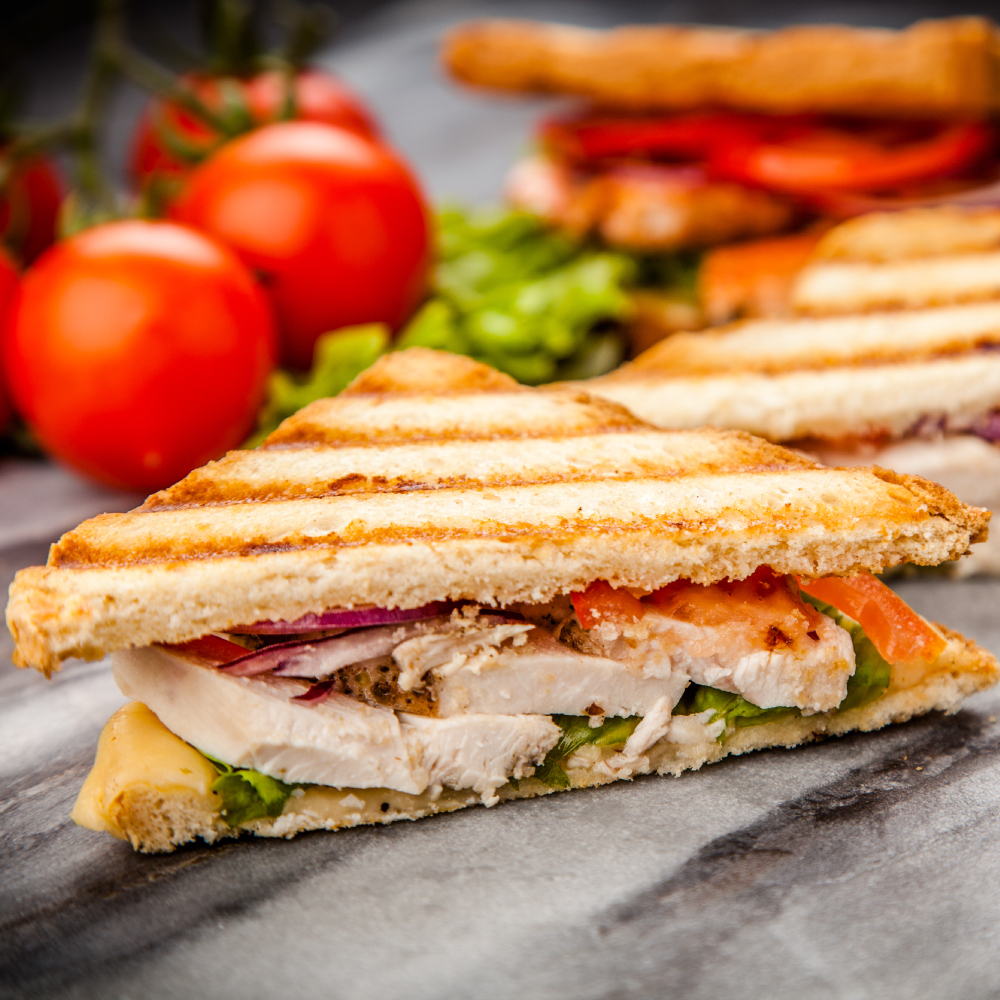
\includegraphics[width=0.5\textwidth]{sandwhich.png}
\end{wrapfigure}

I en sandwichbar viser erfaringen, at 30\,\% af de sandwicher, der bliver solgt, er med kylling.

En dag sælger baren 110 sandwich.

Den stokastiske variabel $X$ betegner antallet af solgte sandwicher, der er med kylling.

Det antages, at $X$ er binomialfordelt med antalsparameter $n=110$ og sandsynlighedsparameter $p=0,30$.

\begin{enumerate}
    \item Bestem sandsynligheden $P(X=29)$, og giv en fortolkning af dette tal.
\end{enumerate}

Et år senere ønsker ejeren af sandwichbaren at undersøge, om andelen af solgte sandwicher med kylling har ændret sig, ved at teste nulhypotesen
\[
    H_0: \text{30 \% af de sandwicher, der bliver solgt, er med kylling.}
\]

Ejeren foretager en stikprøve, og blandt 110 tilfældigt udvalgte solgte sandwicher viser det sig, at 37 af dem er med kylling.

\begin{enumerate}
    \setcounter{enumi}{1}
    \item Bestem acceptområdet for et dobbeltsidet binomialtest på 5 \% signifikansniveau, og afgør, om nulhypotesen kan forkastes.
\end{enumerate}

\end{document}

%%%%%%%%%%%%%%%%%%%%%%%%%%%%%%%%%%%%%%%%%%%%%%%%%%%%%%%%%%%%%%%%%%%%%%%%%%%%%% Skabeloner

% Sidestillet figur
\begin{wrapfigure}[8]{r}{0.2\textwidth}
\vspace{-18pt}
\includegraphics[width=0.3\textwidth]{ovn}
\end{wrapfigure}

% Midterstillet figur
\begin{figure}[h!]
\centering
\includegraphics[width=0.8\textwidth]{abc}
\end{figure}

% Førstillet figur
\
\begin{figure}[h!]
\centering
\vspace{-15pt}
\includegraphics[width=0.35\textwidth]{stud}
\end{figure}

% Tabel
\begin{figure}[h!]
\centering\renewcommand{\arraystretch}{1.5}
\begin{tabularx}{0.9\textwidth}{|l|b|b|b|b|b|b|}
	\hline \cellcolor{hggreen} Decimaltal & 7\% & -51\% & 13,7\% & 126\% & 456\% & 0,28\%\\\hline
	\cellcolor{hggreen} Procenttal &  &  &  &  &  & \\\hline
\end{tabularx}
\end{figure}

% Forklaringsopgaver
\begin{align*}
&&	&						&&\underset{\rule{0.8\linewidth}{0pt}}{\textbf{Forklaring:}}\\[1em]
&&	&\frac{(x+2)^2 - 4}{x} 		&&\underset{\rule{0.8\linewidth}{0.4pt}}{\text{Udtrykket skrives op.}}\\[2em]
&&	=&\ \frac{x^2 + 4 + 4x - 4}{x}	&&\underset{\rule{0.8\linewidth}{0.4pt}}{\text{}}\\[2em]
&&	=&\ \frac{x^2 + 4x}{x}			&&\underset{\rule{0.8\linewidth}{0.4pt}}{\text{}}\\[2em]
&&	=&\ x + 4					&&\underset{\rule{0.8\linewidth}{0.4pt}}{\text{}}\\[2em]
\end{align*}

% Sørg for at figur er placeret før et vidst sted
\FloatBarrier
